%%Trying out a new ordering for the paper.
%%
%% This is file `sample-manuscript.tex',
%% generated with the docstrip utility.
%%
%% The original source files were:
%%
%% samples.dtx  (with options: `manuscript')
%% 
%% IMPORTANT NOTICE:
%% 
%% For the copyright see the source file.
%% 
%% Any modified versions of this file must be renamed
%% with new filenames distinct from sample-manuscript.tex.
%% 
%% For distribution of the original source see the terms
%% for copying and modification in the file samples.dtx.
%% 
%% This generated file may be distributed as long as the
%% original source files, as listed above, are part of the
%% same distribution. (The sources need not necessarily be
%% in the same archive or directory.)
%%
%% The first command in your LaTeX source must be the \documentclass command.
%%%% Small single column format, used for CIE, CSUR, DTRAP, JACM, JDIQ, JEA, JERIC, JETC, PACMCGIT, TAAS, TACCESS, TACO, TALG, TALLIP (formerly TALIP), TCPS, TDSCI, TEAC, TECS, TELO, THRI, TIIS, TIOT, TISSEC, TIST, TKDD, TMIS, TOCE, TOCHI, TOCL, TOCS, TOCT, TODAES, TODS, TOIS, TOIT, TOMACS, TOMM (formerly TOMCCAP), TOMPECS, TOMS, TOPC, TOPLAS, TOPS, TOS, TOSEM, TOSN, TQC, TRETS, TSAS, TSC, TSLP, TWEB.
% \documentclass[acmsmall]{acmart}

%%%% Large single column format, used for IMWUT, JOCCH, PACMPL, POMACS, TAP, PACMHCI
% \documentclass[acmlarge,screen]{acmart}

%%%% Large double column format, used for TOG
% \documentclass[acmtog, authorversion]{acmart}

%%%% Generic manuscript mode, required for submission
%%%% and peer review
\documentclass[manuscript,screen]{acmart}

%%
%% \BibTeX command to typeset BibTeX logo in the docs
\AtBeginDocument{%
  \providecommand\BibTeX{{%
    \normalfont B\kern-0.5em{\scshape i\kern-0.25em b}\kern-0.8em\TeX}}}

%% Rights management information.  This information is sent to you
%% when you complete the rights form.  These commands have SAMPLE
%% values in them; it is your responsibility as an author to replace
%% the commands and values with those provided to you when you
%% complete the rights form.
\setcopyright{acmcopyright}
\copyrightyear{2018}
\acmYear{2018}
\acmDOI{10.1145/1122445.1122456}

%% These commands are for a PROCEEDINGS abstract or paper.
%%\acmConference[Woodstock '18]{Woodstock '18: ACM Symposium on Neural
%%  Gaze Detection}{June 03--05, 2018}{Woodstock, NY}
%%\acmBooktitle{Woodstock '18: ACM Symposium on Neural Gaze Detection,
%%  June 03--05, 2018, Woodstock, NY}
%\acmPrice{15.00}
%\acmISBN{978-1-4503-XXXX-X/18/06}


%%
%% Submission ID.
%% Use this when submitting an article to a sponsored event. You'll
%% receive a unique submission ID from the organizers
%% of the event, and this ID should be used as the parameter to this command.
%%\acmSubmissionID{123-A56-BU3}

%%
%% The majority of ACM publications use numbered citations and
%% references.  The command \citestyle{authoryear} switches to the
%% "author year" style.
%%
%% If you are preparing content for an event
%% sponsored by ACM SIGGRAPH, you must use the "author year" style of
%% citations and references.
%% Uncommenting
%% the next command will enable that style.
%%\citestyle{acmauthoryear}

\usepackage{subcaption}


\DeclareMathOperator{\Div}{div}
\DeclareMathOperator{\curl}{curl}

\newcommand{\R}{\mathbb{R}}
\newcommand{\red}[1]{\textcolor{red}{#1}}
\newcommand{\akg}[1]{\textcolor{blue}{\textbf{AG:} #1}}

\newcommand{\calQ}{\mathcal{Q}}
\newcommand{\calS}{\mathcal{S}}

%%
%% end of the preamble, start of the body of the document source.
\begin{document}

%%
%% The "title" command has an optional parameter,
%% allowing the author to define a "short title" to be used in page headers.
\title{Bringing Serendipity Methods to Computational Practice in Firedrake}

%%
%% The "author" command and its associated commands are used to define
%% the authors and their affiliations.
%% Of note is the shared affiliation of the first two authors, and the
%% "authornote" and "authornotemark" commands
%% used to denote shared contribution to the research.
\author{Cyrus Cheng}
\email{cyrus.cheng15@imperial.ac.uk}
\affiliation{%
  \institution{Imperial College}
  \city{London}
  \country{United Kingdom}
}

\author{Justin Crum}
\email{jcrum@math.arizona.edu}
\affiliation{%
  \institution{University of Arizona}
  \city{Tucson}
  \state{Arizona}
}

\author{Andrew Gillette}
\affiliation{%
  \institution{University of Arizona}
  \city{Tucson}
  \state{Arizona}}
\email{agillette@math.arizona.edu}

\author{David Ham}
\affiliation{%
  \institution{Imperial College}
  \city{London}
  \country{United Kingdom}
}
\email{david.ham@imperial.ac.uk}

\author{Robert Kirby}
\affiliation{%
 \institution{Baylor University}
 \city{Waco}
 \state{Texas}
}
\email{robert_kirby@baylor.edu}

\author{Joshua A. Levine}
\affiliation{%
  \institution{University of Arizona}
}
\email{josh@email.arizona.edu}

\author{Lawrence Mitchell}
\affiliation{%
  \institution{Durham University}
  \city{Durham}
  \country{United Kingdom}}
\email{wence@gmx.li}
%%
%% By default, the full list of authors will be used in the page
%% headers. Often, this list is too long, and will overlap
%% other information printed in the page headers. This command allows
%% the author to define a more concise list
%% of authors' names for this purpose.
%\renewcommand{\shortauthors}{Trovato and Tobin, et al.}

%%
%% The abstract is a short summary of the work to be presented in the
%% article.

\begin{abstract}
    An abstract about Firedrake and FEM here.
  \end{abstract}
  
  
  \maketitle
  
  
  \section{Introduction}
  
  \section{Background on serendipity and trimmed serendipity elements}
  
  \subsection{2D Elements}
  \begin{enumerate}
  \item Scalar (classical = Arnold-Awanou = $\calS_r\Lambda^0(\R^2)$)
  \item Vector Serendipity (BDM = Arnold-Awanou = $\calS_r\Lambda^1(\R^2)$)
  \item Vector Trimmed Serendipity (Arbogast-Correa = Gillette-Kloefkorn = $\calS_r^-\Lambda^1(\R^2)$)
  \item Direct (Arbogast-Tao / Arbogast-Correa)
  \end{enumerate}
  
  
  \subsubsection{Scalar (classical = Arnold-Awanou = $\calS_r\Lambda^0(\R^2)$)}
  
  \subsubsection{Vector Serendipity (BDM = Arnold-Awanou = $\calS_r\Lambda^1(\R^2)$)}
  
  \subsubsection{Vector Trimmed Serendipity (Arbogast-Correa = Gillette-Kloefkorn = $\calS_r^-\Lambda^1(\R^2)$)}
  
  \subsubsection{Direct (Arbogast-Tao / Arbogast-Correa)}
  
  \subsection{3D Elements}
  \begin{enumerate}
  \item Scalar (classical = Arnold-Awanou = $\calS_r\Lambda^0(\R^3)$)
  \item Vector serendipity (Arnold-Awanou = $\calS_r\Lambda^1(\R^3)$ and $\calS_r\Lambda^2(\R^3)$
  \item Vector trimmed serendipity (Gillette-Kloefkorn = $\calS_r^-\Lambda^1(\R^3)$ and $\calS_r^-\Lambda^2(\R^3)$)
  
  \end{enumerate}
  
  \section{Building capacity for serendipity element types in Firedrake}
  
  Firedrake is a python package that is made to solve finite element problems.  It does this by tying together many packages in a cohesive manner.  For implementing a new finite element, we can focus on a few specific packages, namely FIAT, FInAT, UFL, and TSFC.  
  
  \noindent First, we use the UFL package.  This is a symbolic math package that implemented the Unified Form Language in Python.  Specifically, UFL allows Firedrake to specify a PDE in weak form that we then want to solve.  Next, FIAT (FInite element Automatic Tabulator) allows a simple Ciarlet implementation of finite elements that makes the process of adding in new types of elements a relatively simple task.  On the other hand, FInAT (FInAT Is not A Tabulator) is a way to pass symbolic for evaluation of finite elements.  What FInAT gives out can then be handled by a form compiler.  The form compiler that Firedrake uses is TSFC (Two Stage Form Compiler), and is used to take the high level, weak form PDE and turn it into low level code that can be solved.  
  
  \noindent Implementing a new element, like the trimmed Serendipity elements in 2 and 3D, then becomes a matter of adding in a new element code to FIAT, telling UFL what to expect when we call the new element (i.e., what type of shapes does it work on, what dimensions does it work in, what type of element it is), and connecting the dots in FInAT and TSFC.  Starting off in the FIAT portion of the code, we create a new element by making a call to the FiniteElement class.  In this class, we give the relevant information for describing a reference element of the type we're choosing.  For example, we need to give it the number of degrees of freedom on each edge and face, and then we need to build and assign basis functions to each of the degrees of freedom.   Once done, the rest of the code is designed for passing around the new element from library to library.  We import the fiat element to FInAT so that it knows of the existence of the new element.  Then we tell TSFC where to find the new element, and give it a name that a Firedrake user can give when calling the element.  Finally, we give UFL the directions of what sort of elements we are allowed to use the new finite element on.    
  

  \section{Experiments}
    
   The following experiments were designed to show the benefits and costs to using trimmed Serendipity elements in comparison to traditional tensor product elements.  We used a basic projection example to check implementation, as well as a primal Poisson problem (to test scalar elements), a mixed Poisson problem (to test H(div) elements), and a cavity resonator problem (to test H(curl) elements).  Note that the cavity resonator problem was done only in 3D, as in 2D, the H(curl) elements are just a rotation of the H(div) elements. 

\newpage
  \subsection{Projection}
  
  We solve the projection problem to give a baseline of expectations for the elements.  
  
  GET THE EXACT PROBLEM THAT THE PROJECTION PROBLEM IS SOLVING.

  \begin{figure}[h!]
    \caption{Analysis of projection using $S^-(\text{Curl})$ and RTCE.}
    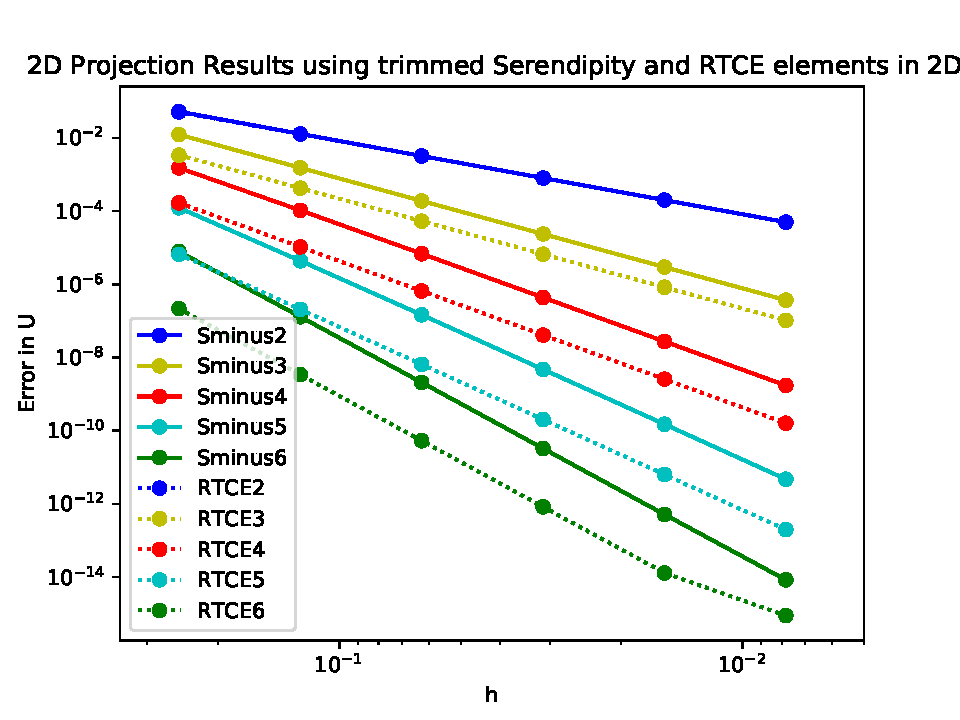
\includegraphics[width=0.55\textwidth]{2dProjectionH.pdf}
    \label{fig:2dProjectionH}
  \end{figure}
  
  \noindent First, we graphed the errors from computing projections using trimmed Serendipity and tensor product elements in 2D, shown in Figure \ref{fig:2dProjection}.  Since we expect that the order of convergence for both of these elements should be the same (only off by a constant factor), we look for the lines representing trimmed Serendipity and tensor product elements at a given order to be parallel.

  \begin{figure}[h!]
    \caption{Degrees of Freedom vs Error analysis of projection using $S^-(\text{Curl})$ and RTCE.}
    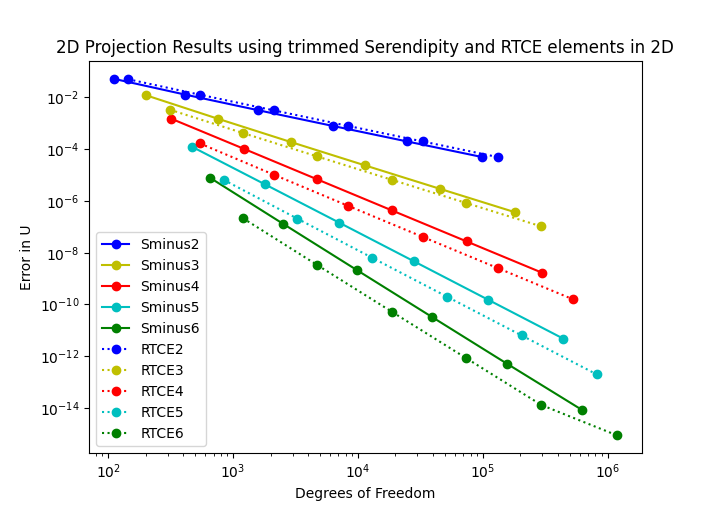
\includegraphics[width=0.55\textwidth]{2dProjection.png}
    \label{fig:2dProjection}
  \end{figure}
  
  \noindent After checking that it is converging at the right rate, we then want to analyze the data from a standpoint of memory usage.  To do this, we plot degrees of freedom vs error, as seen in Figure \ref{fig:2dProjection}.  Overall, the error given by trimmed Serendipity elements is higher than the error from using tensor product elements of the same order.  However, the degrees of freedom comparison allows us to instead compare error per degree of freedom, which tends to favor trimmed Serendipity elements at higher degrees.  To see this in a few more practical (but still relatively simple problems), we move on to the next few experiments.
  


\newpage
  \subsection{Primal Poisson}
  
\noindent We solve the primal Poisson problem described below on a unit square domain $\Omega$
\begin{align}
    -\nabla^2 u &= f \\
    u\vert_{\partial \Omega} &= 0 \\
    \nabla u \cdot n &= 0 \text{ on } \partial \Omega
\end{align}
where $f(x,y) = 2\pi^2\text{sin}(\pi x)\text{sin}(\pi y) $, yielding the solution $u(x,y) = \text{sin}(\pi x)\text{sin}(\pi y)$. In 3D, we can extend this to $f(x,y,z) = 2\pi^2\text{sin}(\pi x)\text{sin}(\pi y)\text{sin}(\pi z)$ with the solution being $u(x,y,z) = \text{sin}(\pi x)\text{sin}(\pi y)\text{sin}(\pi z)$.  

\begin{figure}[h!]
  \centering
  \begin{subfigure}[h]{0.5\textwidth}
    \centering
    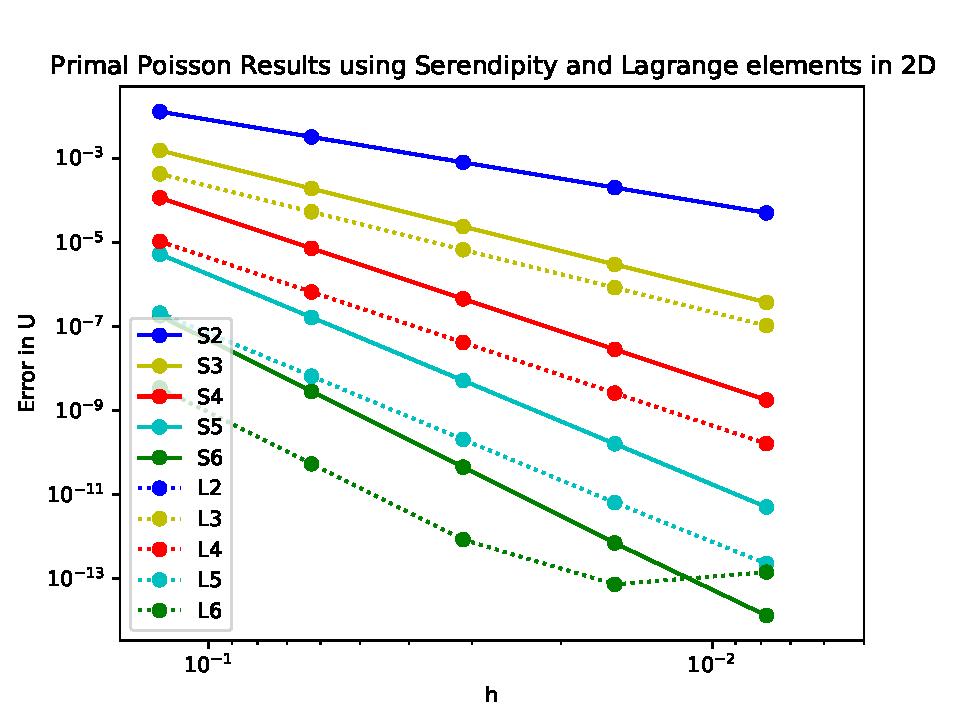
\includegraphics[height=2.2in]{2dPrimalH.pdf}
    \caption{2D}
    \label{fig:2dPrimalH}
  \end{subfigure}
  ~
  \begin{subfigure}[h]{0.5\textwidth}
    \centering
    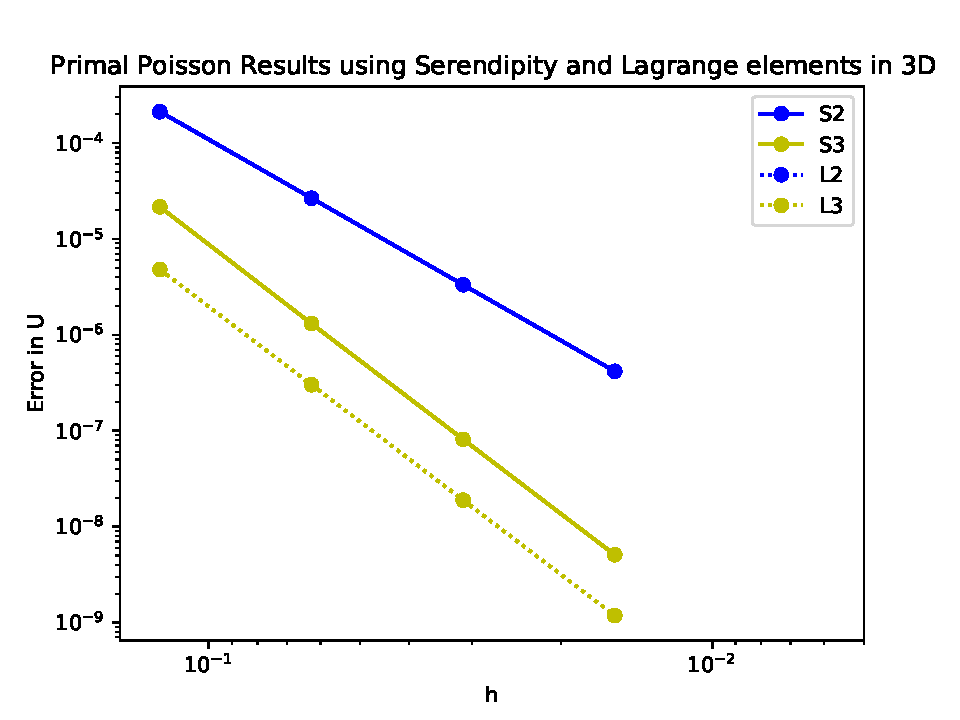
\includegraphics[height=2.2in]{3dPrimalH.pdf}
    \caption{3D}
    \label{fig:3dPrimalH}
  \end{subfigure}
  \caption{Analysing the error based off the mesh refinements for the primal Poisson problem in 2 and 3D.}
\end{figure}  
\noindent  As in the projection problem, we first give Figures \ref{fig:3dPrimalH} and \ref{fig:2dPrimalH} to illustrate the behavior of these elements with respect to mesh refinement.  In general, Lagrange elements again give better error with respect to mesh refinement (ignoring order 6 in 2D when getting close to machine precision).  In 3D, we focus on orders 2 and 3, as even in this case, we hit approximately 1TB of memory used and require nearly 12 hours of computation time on 24 processors.

\noindent Though the Lagrange elements tend to give a better error approximation at each mesh refinement level, we also wish to investigate the cases of how much error can we get if we instead wish to limit the amount of memory or time that the machine uses.  In Figures \ref{fig:2dPrimalDofs} and \ref{fig:3dPrimalDofs}, we have trendlines illustrating the degrees of freedom in the mesh vs the error.  What we find is that at the lower orders (order 2 for 2D and both orders 2 and 3 for 3D), the Serendipity curves show a better error  at the same degrees of freedom, while the Lagrange elements overtake them at higher orders.  

\begin{figure}[h!]
  \centering
  \begin{subfigure}[h]{0.5\textwidth}
    \centering
    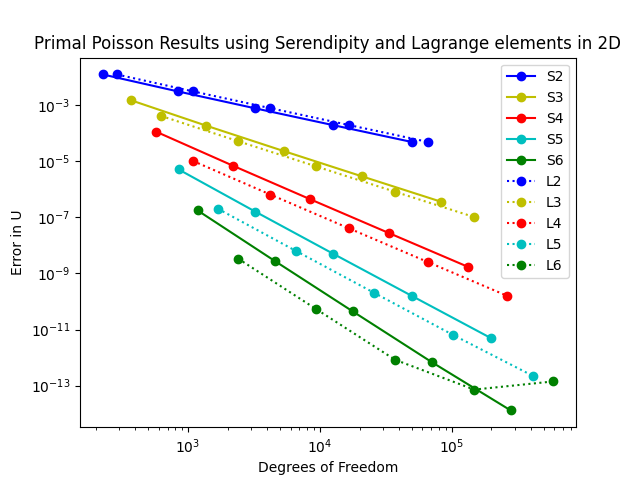
\includegraphics[height=2.2in]{2dPrimalPoisson.png}
    \caption{2D}
    \label{fig:2dPrimalDofs}
  \end{subfigure}
  ~
  \begin{subfigure}[h]{0.5\textwidth}
    \centering
    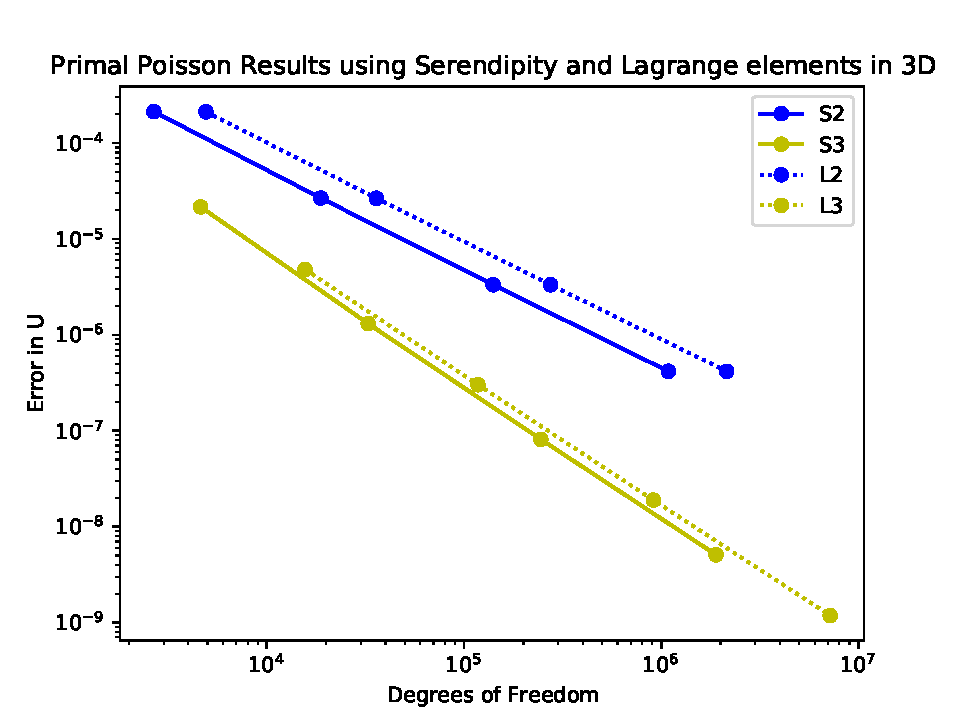
\includegraphics[height=2.2in]{3dPrimalDofs.pdf}
    \caption{3D}
    \label{fig:3dPrimalDofs}
  \end{subfigure}
  \caption{Analyzing the primal Poisson problem in 2 and 3D based off degrees of freedom vs error.}
\end{figure}  

%  \begin{figure}[h!]
%    \caption{Degrees of Freedom vs Energy Error analysis of Serendipity and Lagrange $L^2$ %elements.}
%    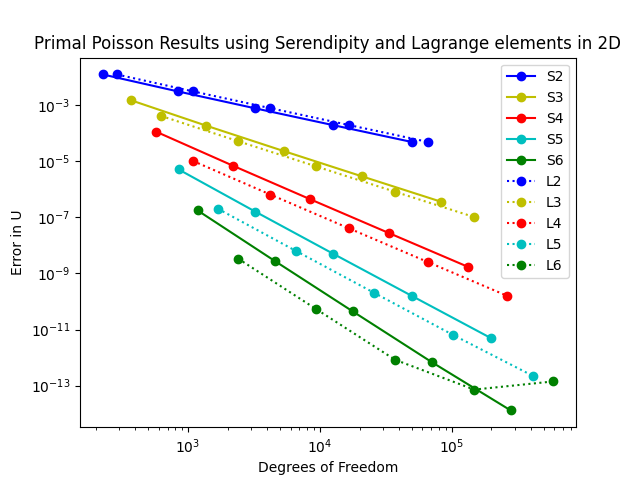
\includegraphics[width=0.75\textwidth]{2dPrimalPoisson.png}
%    \label{fig:2dPrimalPoisson}
%  \end{figure}

%  \begin{figure}[h!]
%    \caption{Degrees of Freedom vs Energy Error analysis of Serendipity and Lagrange $L^2$ %elements.}
%    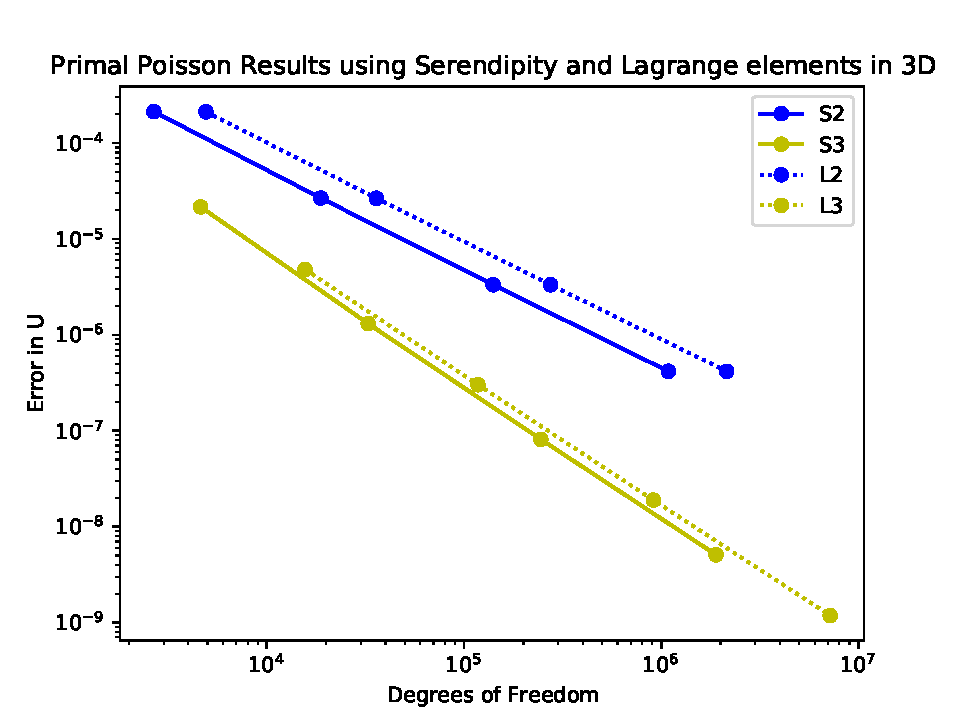
\includegraphics[width=0.75\textwidth]{3dPrimalDofs.pdf}
%    \label{fig:3dPrimalDofs}
%  \end{figure}

  \begin{figure}[h]
    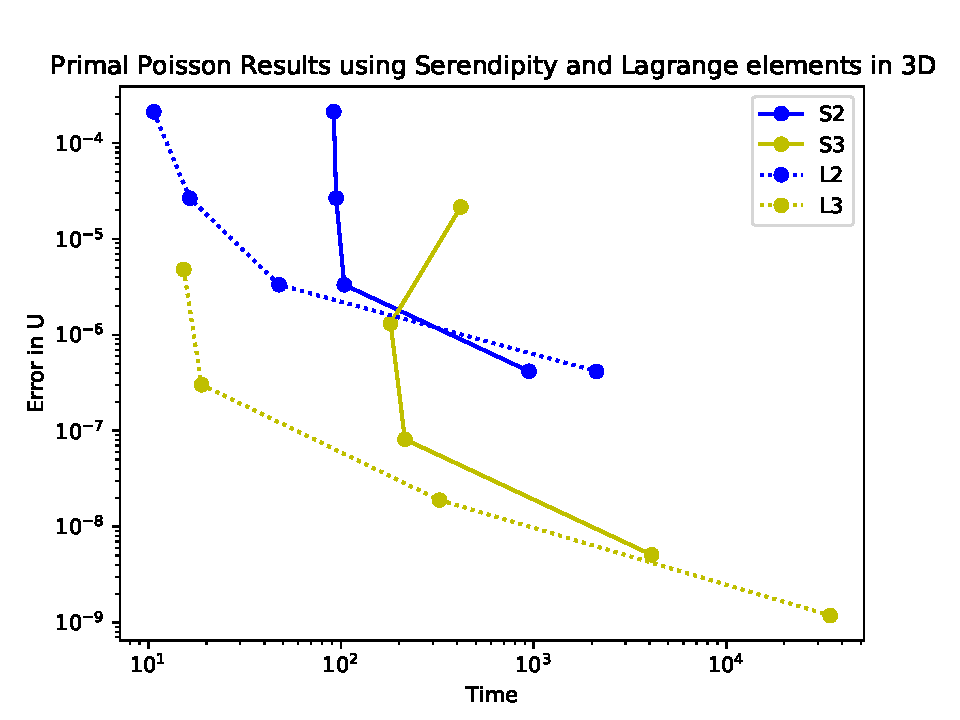
\includegraphics[width=0.55\textwidth]{3dPrimalTime.pdf}
    \caption{Timing data for the 3D primal Poisson problem, where each sequence of data represents using the respective element for a mesh of size $N x N x N$ for $N = 8, 16, 32, 64$.}
    \label{fig:3dPrimalTime}
  \end{figure}
\newpage 

\noindent Finally, we look at the timing requirements for the primal Poisson problem using the Lagrange and Serendipity elements in 3D.  In \ref{fig:3dPrimalTime}, we can see that the amount of time required for Serendipity elements tends to start off higher, but scales better as the problem grows in size.  


\newpage
\subsection{Mixed Poisson}

  
The mixed Poisson problem that we focus on is derived from the primal Poisson equation above.  Specifically, we solve a discretization of 

\begin{align}
     \sigma - \nabla u &= 0 \\
     \nabla \cdot \sigma &= -f \notag \\
     u\vert_{\partial \Omega} &= 0 \notag
\end{align}

 
%\begin{equation}
%%    \sigma - \nabla u = 0
%\end{equation}
%\begin{equation*}
%    \nabla \cdot \sigma = -f
%\end{equation*}
%\begin{equation*}
%    u\vert_{\partial \Omega} = 0
%\end{equation*}

\noindent which has the same analytic 2 and 3D solutions as the primal Poisson problem when using $f$ as defined in section 4.2.  The error results based off mesh refinements can be seen in Figures \ref{fig:2dMixedPoissonH} and \ref{fig:3dMixedPoissonH}.  The 2D mixed Poisson graph is similar to the 2D primal Poisson graph.  The 3D mixed Poisson graph again illustrates the proper rates of convergence for trimmed Serendipity elements, but also illustrates the computational difficulty of scaling the tensor product elements to larger problems in 3D.

\begin{figure}[h!]
  \centering
  \begin{subfigure}[h]{0.5\textwidth}
    \centering
    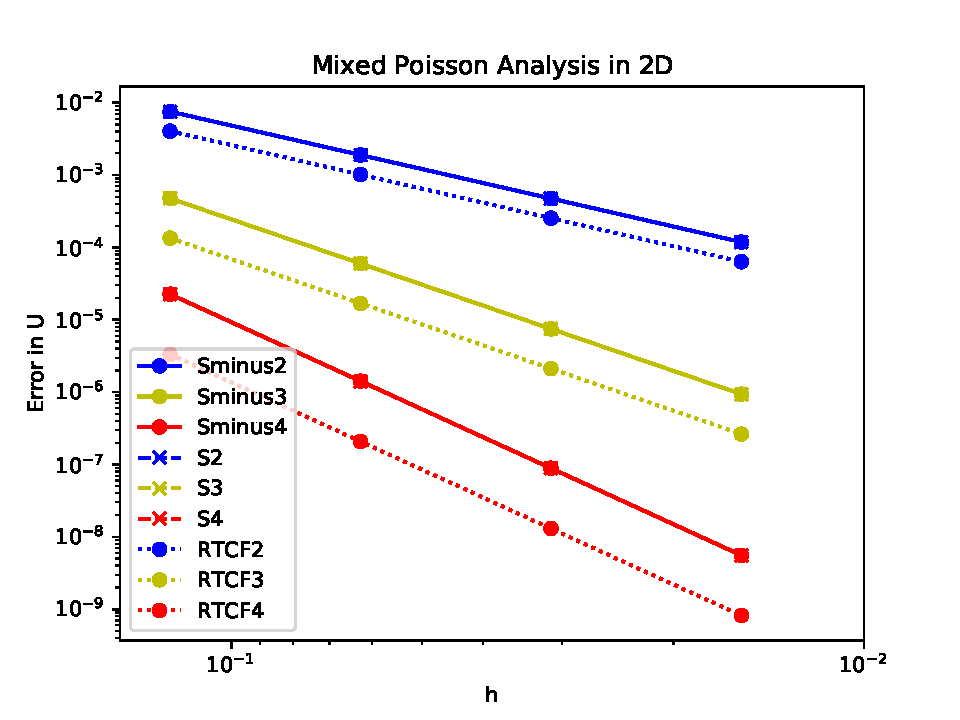
\includegraphics[height=2.2in]{2dMixedPoissonH.pdf}
    \caption{2D}
    \label{fig:2dMixedPoissonH}
  \end{subfigure}
  ~
  \begin{subfigure}[h]{0.5\textwidth}
    \centering
    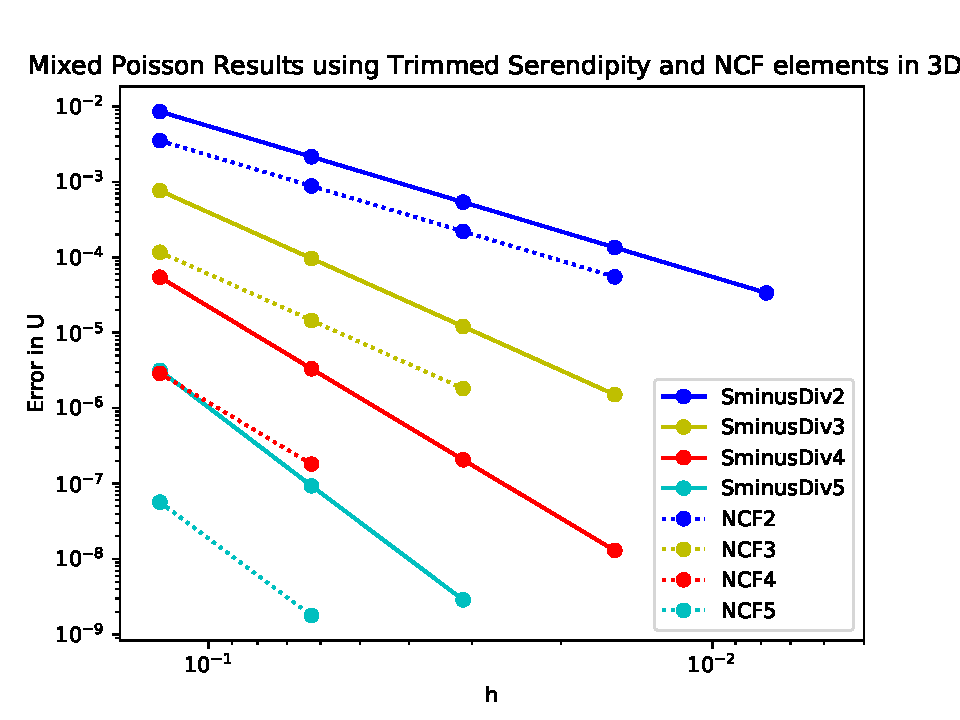
\includegraphics[height=2.2in]{3dMixedPoissonH.pdf}
    \caption{3D}
    \label{fig:3dMixedPoissonH}
  \end{subfigure}
  \caption{Analyzing the mixed Poisson problem in 2 and 3D based off edge length $h$ vs error.}
\end{figure} 

%  \begin{figure}[h!]
%    \caption{Degrees of Freedom vs h analysis of $S^-(\text{Div})$ and RTCE elements for a %mixed Poisson PDE, with exact solution $sin(\pi x)sin(\pi y)$ !}
%    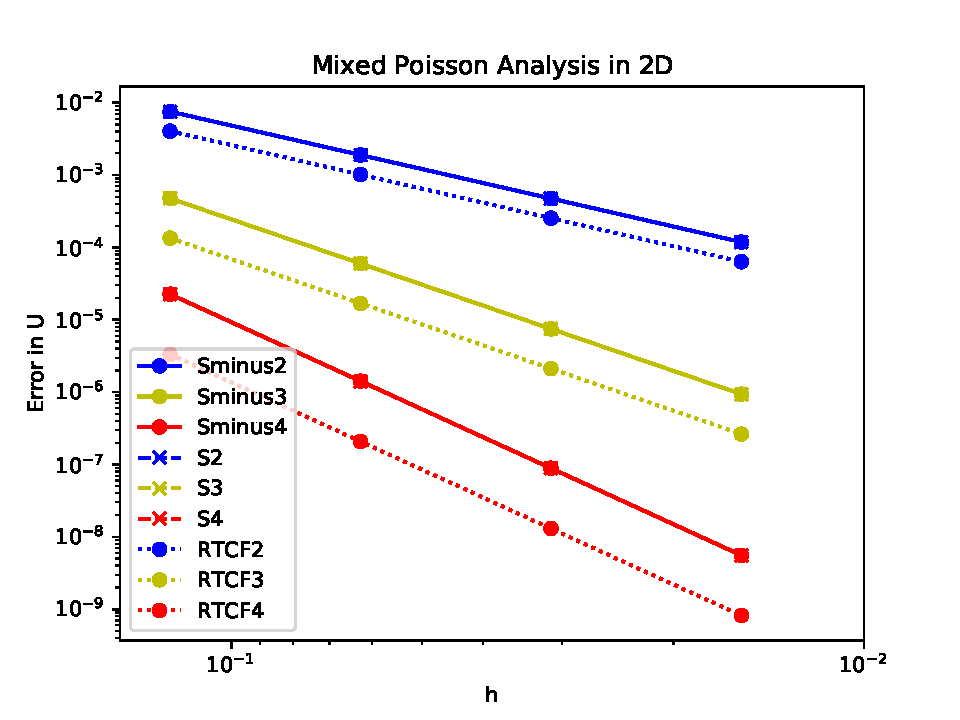
\includegraphics[width=0.75\textwidth]{2dMixedPoissonH.pdf}
%    \label{fig:2dMixedPoissonH}
%  \end{figure}

\newpage

\noindent After the comparison based off edge length, we also want to focus on the error based on the degrees of freedom.  In Figures \ref{fig:2dMixedDofs} and \ref{fig:3dMixedDofs}, we see similar trends to our previous figures.

\begin{figure}[h!]
  \centering
  \begin{subfigure}[h]{0.45\textwidth}
    \centering
    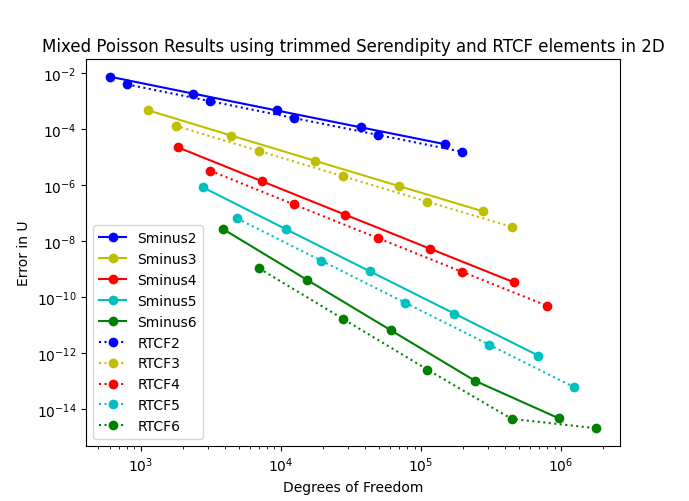
\includegraphics[height=2.1in]{MixedPoisson-2d-SminusDiv_RTCF.png}
    \caption{2D}
    \label{fig:2dMixedDofs}
  \end{subfigure}
  ~
  \begin{subfigure}[h]{0.45\textwidth}
    \centering
    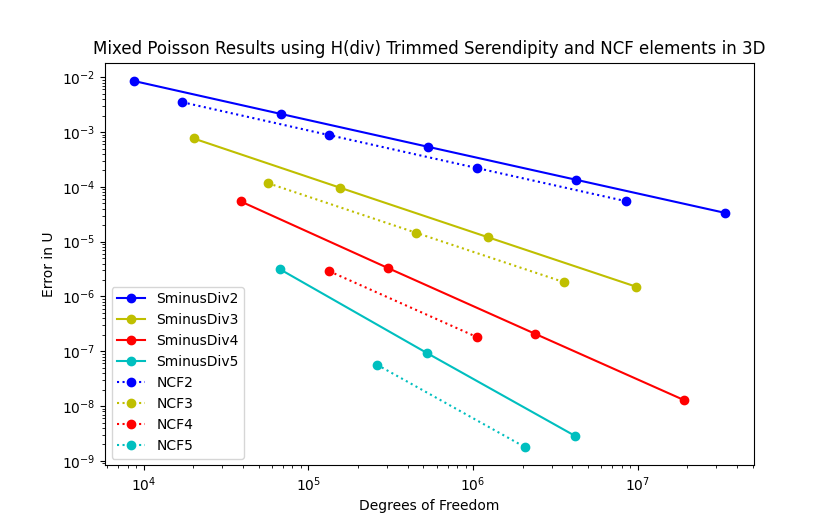
\includegraphics[height=2.1in]{MixedPoisson3d_TrimmedSerendipityNCF.png}
    \caption{3D}
    \label{fig:3dMixedDofs}
  \end{subfigure}
  \caption{Analyzing the mixed Poisson problem in 2 and 3D based off degrees of freedom vs error.}
\end{figure} 

\newpage

%  \begin{figure}[h!]
%    \caption{Degrees of Freedom vs Error analysis of $S^-(\text{Div})$ and RTCE elements for %a mixed Poisson PDE, with exact solution $sin(\pi x)sin(\pi y)$ !}
%    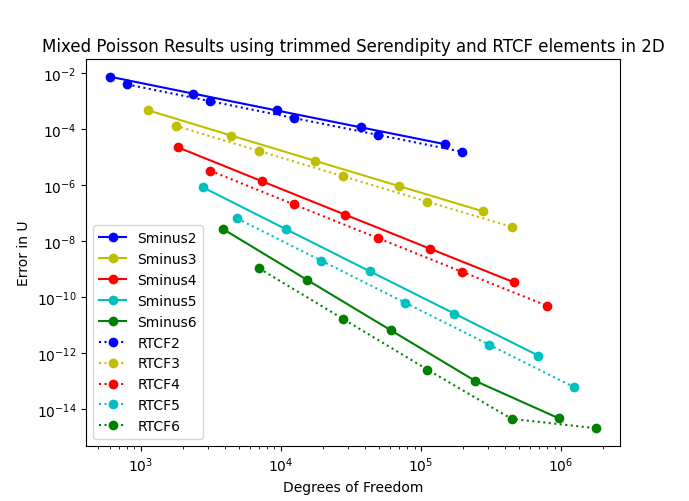
\includegraphics[width=0.75\textwidth]{MixedPoisson-2d-SminusDiv_RTCF.png}
%    \label{fig:2dMixedPoisson}
%  \end{figure}

%  \begin{figure}[h]
%    \caption{Preliminary results for testing a mixed Poisson problem in 3D, using %$S^-(\text{Div})$ and NCF elements.}
%    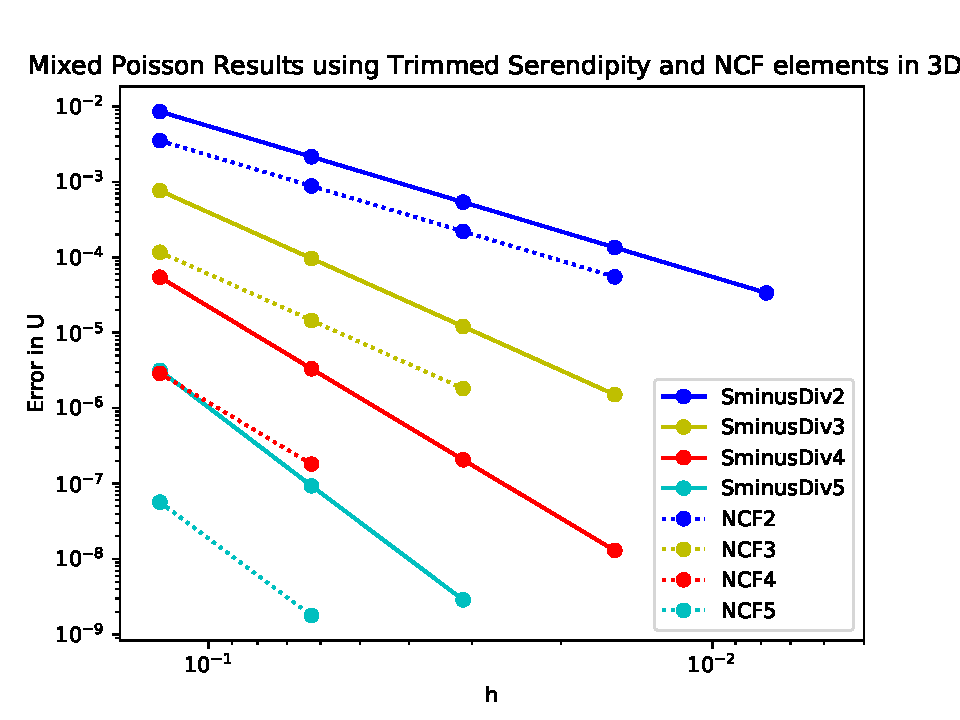
\includegraphics[width=0.75\textwidth]{3dMixedPoissonH.pdf}
%  \caption{Analyzing convergence rates of trimmed Serendipity vs tensor product elements in %3D using H$($div$)$ elements.}
%  \label{fig:3dTrimmedDivN}
%  \end{figure}

%  \begin{figure}[h!]
%    \caption{Preliminary results for testing a mixed Poisson problem in 3D, using %$S^-(\text{Div})$ and NCF elements.}
%    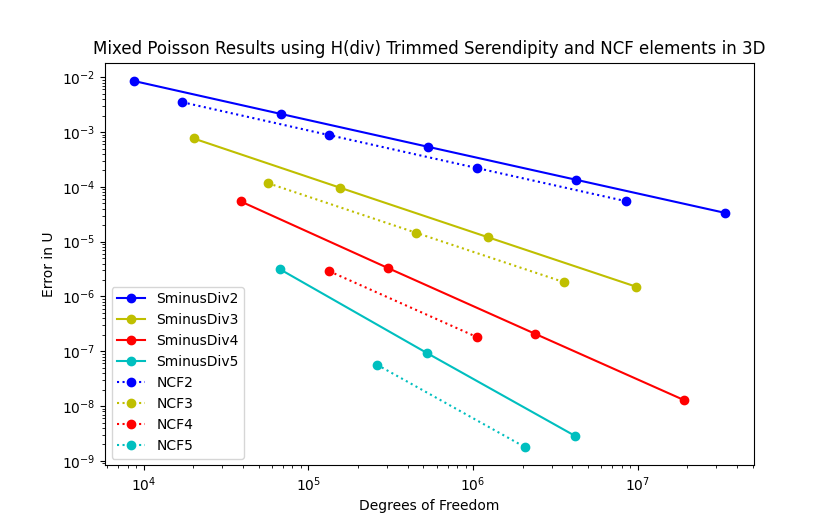
\includegraphics[width=0.75\textwidth]{MixedPoisson3d_TrimmedSerendipityNCF.png}
%  \caption{Analyzing convergence rates of trimmed Serendipity vs tensor product elements in %3D using H$($div$)$ elements.}
%  \label{fig:3dTrimmedDiv}
%  \end{figure}

  \subsection{Cavity Resonator}

\noindent For testing the H$($curl$)$ elements in 3D, we use the cavity resonator problem.  Here, the time-harmonic Maxwell equations are applied to a domain $\Omega = [0,1]^3$ with perfectly conducting boundary conditions, yielding an eigenvalue problem where $\omega$ represents the resonances (i.e.\ eigenvalues) and $E$ represents the electric field (i.e.\ eigenfunctions):


\begin{equation}
    \langle \text{curl}(F), \text{curl}(E) \rangle = \omega^2 \langle F, E \rangle \text{ for all } F \in H_0(\text{curl}).
\end{equation}

%\noindent We tested out the H$($curl$)$ elements in 3D on the cavity resonator problem, where the time-harmonic Maxwell equations applied to a 
%\akg{(1) The wording is a little ambiguous - are you about the state the resonator problem or Maxwell's equations?  Or are these the same?  (2) I prefer to see the statement of the variables prior to the PDE i.e. move the part after the equation to before it. (3) You need to state the domain - I think it's $[0,1]^3\subset\R^3$ - and the boundary conditions (periodic?) (4) Give the eigenvalue equation a label so you can reference it later.}

\noindent The exact eigenvalues should follow the formula

\[ \omega^2 = m_1^2 + m_2^2 + m_3^2 \]

\noindent where $m_i \in \mathbb{N} \cup {0}$ and no more than one of $m_1, m_2, m_3$ may be equal to $0$ at a time \cite{rognes2010efficient}.

%\akg{Put discretized version of eigenvalue problem here (see comment below)}

\begin{center}
\begin{table}
\begin{tabular}{ c c c c c }
\multicolumn{5}{c}{NCE Elements} \\
\hline
Actual & N = 4 & N = 8 & N = 16 & N = 32 \\ 
\hline
2 &2.0010243 & 2.0000655 (3.97) & 2.0000041 (3.99) & 2.0000003 (4.00) \\  
2 & 2.0010243 & 2.0000655 (3.97) & 2.0000041 (3.99) & 2.0000003 (4.00)  \\
2 & 2.0010243 & 2.0000655 (3.97) & 2.0000041 (3.99) & 2.0000003 (4.00)\\
3 & 3.0015364 & 3.0000983 (3.97) & 3.0000062 (3.99) & 3.0000004 (4.00) \\
3 & 3.0015364 & 3.0000983 (3.97) & 3.0000062 (3.99) & 3.0000004 (4.00) \\
$! \rightarrow$ 4 & 4.0300893 & 4.0020486 (3.88) & 4.0001311 (3.97) & 4.0000082 (3.99) \\
$! \rightarrow$ 4 & 4.0300893 & 4.0020486 (3.88) & 4.0001311 (3.97) & 4.0000082 (3.99) \\
5 & 5.0306014 & 5.0020813 (3.88)& 5.0001331 (3.97) & 5.0000084 (3.99) \\
5 & 5.0306014 & 5.0020813 (3.88)& 5.0001331 (3.97) & 5.0000084 (3.99) \\
5 & 5.0306014 & 5.0020813 (3.88) & 5.0001331 (3.97) & 5.0000084 (3.99) \\
5 & - & - & 5.0001331 & 5.0000084 (3.99) \\
6 & - & 6.0021141 & 6.0001352 (3.97) & -  \\
6 & - & 6.0021141 & 6.0001352 (3.97) & - \\
\hline
DOF  & 1944 & 13872 & 104544 & 811200 \\
\hline
EPS Solve Time (seconds) & 0.0514 & 0.2811 & 3.2795 & 29.2620 \\
\hline
\multicolumn{5}{c}{$S^-$ H$($curl$)$ Elements} \\
\hline
Actual & N = 4 & N = 8 & N = 16 & N = 32 \\ 
\hline
2 &2.0010919 & 2.0000664 (4.04) & 2.0000041 (4.01) & 2.0000003 (4.00) \\  
2 & 2.0010919 & 2.0000664 (4.04) & 2.0000041 (4.01) & 2.0000003 (4.00)  \\
2 & 2.0059537 & 2.0003900 (3.93) & 2.0000247 (3.98) & 2.0000015 (4.00)\\
3 & 3.0090182 & 3.0005863 (3.94) & 3.0000370 (3.98) & 3.0000023 (4.00) \\
3 & 3.0090182 & 3.0005863 (3.94) & 3.0000370 (3.98) & 3.0000023 (4.00) \\
$! \rightarrow$ 4 & 4.0300893 & 4.0020486 (3.88) & 4.0001311 (3.97) & 4.0000082 (3.99) \\
$! \rightarrow$ 4 & 4.0300893 & 4.0020486 (3.88) & 4.0001311 (3.97) & 4.0000082 (3.99) \\
5 & 5.0320266 & 5.0020970 (3.93)& 5.0001333 (3.98) & 5.0000084 (3.99) \\
5 & 5.0320266 & 5.0020970 (3.93)& 5.0001333 (3.98) & 5.0000084 (3.99) \\
5 & 5.0736899 & 5.0052310 (3.82) & 5.0001333 (5.29) & 5.0000212 (2.65) \\
5 & 5.0736899 & 5.0052310 (3.82) & 5.0003371 (3.96) & 5.0000212 (3.99) \\
6 & - & 6.0049765 & 6.0003192 (3.96) & 6.0000201 (3.99) \\
6 & - & - & - & - \\
\hline
DOF  & 1080 & 7344 & 53856 & 411840 \\
\hline
EPS Solve Time (seconds) & 0.0367 & 0.1339 & 1.5125 & 17.6765 \\
\hline

\end{tabular}
\caption{A comparison of how order 2 NCE and $S^-$ finite elements solve the Maxwell cavity resonator eigenvalue problem, $\langle \text{curl}(F), \text{curl}(E) \rangle = \omega^2 \langle F, E \rangle$. }  
\label{tab:Eigenvalue}
\end{table}
\end{center}

%\akg{(1) For this second paragraph, the first (topic) sentence is good - you are going to discuss the table.  The next few sentences need to be *what* the table is.   What are the columns?  What are the rows?  What is the top vs the bottom of the table?  What does each entry in the table represent?  What is in the parentheses?  *Then* give the formula for convergence rate, and explain what the !-4 notation means, and the specifics about SLEPc. Imagine you are teaching this to a first year graduate student - you have to explain everything.  That should be the entire content of this paragraph.  Then have a new paragraph with topic sentence something like ``Table~\ref{tab:Eigenvalue} highlights a number of revealing differences between computing with NCE and serendipity elements.''  Then launch into what those differences are.
%(2) FYI: I added `Table' before the ref command.  Also I had to move the label command before the end table command as it was picking up the section number instead of the table number.  
%(3) You're not *really* solving the eigenvalue problem - you're solving a discretization of it.   I think we need to state the discretized version formally.  We can discuss this when we talk if  you're not sure how / where to find the formulation.   }

\noindent In Table~\ref{tab:Eigenvalue}, we look at the convergence rates of different eigenvalues based off solving the problem with tensor product (NCE) elements and trimmed Serendipity ($S^-$) elements in 3D.  The table is split into two mirrored halves, the top half giving values from using NCE elements while the bottom half gives values from using $S^-$ elements.  The column labeled "Actual" represents the theoretical eigenvalue that eigenvalues in that row are converging towards.  Each of the $N=4, N=8, N=16, N=32$ columns represents the approximate eigenvalues calculated on a mesh of size $N x N x N$.  The number in parenthesis next to approximate eigenvalues is the rate of convergence of that eigenvalue.  Finally, each half has a row giving the overall degrees of freedom in the mesh at each given mesh size and another row that gives the time that the eigenvalue solver needed to find the requested number of eigenvalues.


\noindent Note that the convergence rates are computed by doing

\[r = \frac{\text{log}\bigg(\frac{\tilde{\lambda}_{i,N} - \lambda_{i,N}}{\tilde{\lambda}_{i,N+1} - \lambda_{i,N+1}} \bigg)}{\text{log}\bigg( \frac{h_N}{h_{N+1}} \bigg)} \]

\noindent and are indicated in the chart by using parentheses.  We use H$($curl$)$ to solve the problems, corresponding with edge elements in 3D.  Based off earlier eigenvalue works \cite{boffi2010finite}, we expect that the rate of convergence be double the order of the finite element used to solve the problem.  This is reflected in the table in most spots, except for one of the eigenvalues of $5$, where it tends to oscillate a bit.  This specific eigenvalue overall converges at a rate near $4.00$ if we instead using the values at $N=8$ and $N=32$, ignoring the intermediate value at $N=16$.  \\

\noindent Based off the closed form formula, note that $4$ should never be an eigenvalue in 3D. However, we see it consistently found by both the NCE and $S^-$ elements.  Any eigenvalue that has a $-$ spot is to be interpreted as the eigenvalue solver did not find that specific eigenvalue in the number of iterations it required to find the first 15 requested eigenvalue-eigenvector pairs.\\

\noindent Knowing that both elements are solving this problem in a fashion that is expected theoretically, we can analyze the rest of the results shown in this table.  Investigating the error in the eigenvalues in the chart compared to the exact values, we see that NCE elements are able to get results that are up to a magnitude better, though not for every eigenvalue.  However, this loss of accuracy from the trimmed Serendipity elements is made up for by the comparison of the DOFs and solve time required.  At every mesh refinement level, trimmed Serendipity elements have nearly half the DOFs of NCE elements, and correspondingly, require about half the time to solve for the eigenvalues.  At higher orders, we expect that this will be even more exaggerated.  \\

\noindent The experiment was done by using SLEPc in Firedrake, computing an inverted shift to a target of $3.0$, then asking SLEPc for $15$ eigenvalue-eigenvector pairs.  SLEPc was then give a tolerance level of $1\text{e}-7$, and then a couple of specific mumps parameters (icntl 14 set to 200 and icntl 13 set to 1).  We ignored the eigenvalues of $1$, as they correspond only to the boundary conditions. 

\section{Conclusion}

\noindent Each finite element has a time and place where it could be considered beneficial to use.  We explored the numerical properties of trimmed Serendipity elements to refine our understanding of how they act.  From the theory, we knew that trimmed Serendipity elements should be able to converge at the same rate as tensor product and Serendipity elements, while using fewer degrees of freedom overall.  The plots here demonstrate that the rate of convergence is consistent with what we expect at many orders for H$($curl$)$, H$($div$)$, and $L^2$ elements in both 2 and 3D.\\

\noindent Beyond the convergence rates hitting what we expect, we were able to analyze memory usage on these problems by studying the degrees of freedom required.  Trimmed Serendipity, while generally have a worse error at a given order $k$, also uses significantly fewer degrees of freedom.  This is illustrated well in the Maxwell Cavity Eigenvalue problem in \ref{tab:Eigenvalue}, where the degrees of freedom required were nearly half of what the tensor product elements used.  \\

\noindent Another example of this is the 3D mixed Poisson problem, where we see that the trimmed Serendipity elements are able to be used at more refined meshes while the tensor product elements would need to be allotted more time on a high memory computer to be able to get results on the same sized mesh.  \\

\noindent In general, it is clear from these results that trimmed Serendipity is not always a better choice compared to tensor product elements.  However, these examples illustrates the benefit of trimmed Serendipity elements--in a setting where the mesh is fixed, the option to use a trimmed Serendipity element might give an extra way to refine a problem to increase the accuracy of a solution.


\bibliographystyle{ACM-Reference-Format}  %Might need acmart.cls (unclear)
\bibliography{serendipityFiredrakePaper}  %Change this to the bib file

\end{document}